\documentclass[a4paper,12pt]{article}
\usepackage[utf8]{inputenc}
\usepackage{mathtools}
\usepackage[spanish]{babel}
\usepackage{appendix}
\usepackage[a4paper]{geometry}



% Allow the change of line spacing
\usepackage{setspace}
\usepackage{tabularx}
\usepackage{graphicx}
\usepackage{underscore}


%\usepackage{hyperref}
%\usepackage{breakurl}

%opening
%\title{Trainmining}
%\author{Grupo de Sistemas Inteligentes \\ Universidad Politécnica de Madrid}


\begin{document}


\include{report1titlepage}
%\maketitles

\section{Resumen del trabajo realizado}
En este primer hito del proyecto, se ha conseguido implementar los 7 filtros necesarios para la implementación del sistema ecualizador en el que consiste nuestro proyecto. Los filtros digitales IIR de orden 2 se han implementado siguiendo las indicaciones del manual de LSED del curso 2011-2012, en el que se indicaba la estructura a seguir y los coeficientes necesarios para cada filtro.

Para la representación de las señales, se ha elegido un ancho de palabra de 16 bits, correspondiente a 6 bits enteros y 10 fraccionarios. Esta elección causa que los errores de cuantificación no sean todo lo pequeños que podrían ser utilizando palabras de 16 bits, pero es una elección segura para evitar problemas de desbordamiento de registros en puntos intermedios del sistema. No obstante, debido a las características de la implementación en VHDL, esta elección podría cambiarse fácilmente en etapas posteriores del proyecto si fuese necesario, gracias a la característica modular de la implementación.

Tras leer varias fuentes de documentación disponibles en internet, se ha optado por utilizar la librería \emph{ieee.numeric_std} en lugar de las librerías \emph{ieee.std_logic_arith} y \emph{ieee.std_logic_signed}. La librería numeric_std proporciona los mismos recursos que las otras dos mencionadas, con la ventaja de que permite fácilmente trabajar al mismo tiempo con números enteros y palabras binarias. Es importante destacar que debido a ello, nuestro tipo de datos no será \emph{std_logic_vector}, sino señales de tipo \emph{signed}. El tipo signed corresponde simplemente a un std_logic_vector en el que además se indica específicamente que es de tipo signed. Esto nos permite realizar operaciones aritméticas directamente sin tener declarar todas nuestras palabras como signed, como ocurre si utilizamos la librería std_logic_signed. Esta elección no supone ningún cambio sustancial respecto a las indicaciones dadas en clase sobre el uso de std_logic_vector, ya que internamente las representaciones de los datos son equivalentes.

Para la implementación de los filtros, se han barajado dos opciones. La primera posibilidad consistía en implementar los 7 filtros como 7 componentes distintos, cada uno con sus coeficientes programados directamente en el código. La segunda posibilidad consistía en implementar un filtro genérico, al que le podamos ajustar sus coeficientes cuando lo utilicemos para implementar el banco de filtros en posteriores hitos. Esta segunda opción nos permite realizar modificaciones (por ejemplo, en el ancho de palabra) fácilmente sin tener que modificar más que un fichero, por lo que se ha optado por ella para la implementación de los filtros. Por tanto, se ha implementado un único componente que corresponde al filtro genérico, que posteriormente se ha importado en un banco de pruebas en el que se han creado 7 instancias del mismo asignando los coeficientes correspondientes.



\section{Resultados y validacion}

Para comprobar la validez de los filtros implementados, se ha creado un banco de pruebas en el que se han creado 7 instancias de filtros. Como se ha mencionado anteriormente, los coeficientes se especifican en cada implementación del filtro mediante el uso de genéricos, por lo que solo tenemos un componente filtro que se instancia 7 veces.

Para comprobar que el funcionamiento de los filtros es el deseado, nos ayudaremos de la herramienta \emph{MATLAB}, que nos permite fácilmente realizar filtros dados los coeficientes \emph{a} y \emph{b} de los que disponemos. En primer lugar, obtendremos sus respuestas al impulso colocando en la simulación a la entrada una función $\delta[n]$. Posteriormente realizaremos la misma operación en MATLAB y comprobaremos que ambas respuestas sean iguales.

En las figuras \ref{fig:filter0}, \ref{fig:filter1}, \ref{fig:filter2}, \ref{fig:filter3}, \ref{fig:filter4}, \ref{fig:filter5} y \ref{fig:filter6} se pueden ver las comprobaciones realizadas. Para cada filtro, se ha representado: La respuesta al impulso obtenida en la simulación con ModelSim (arriba a la izquierda); la respuesta al impulso obtenida con MATLAB (arriba a la derecha); y la diferencia en valor absoluto de ambas señales (debajo).

La señal de la simulación de ModelSim ha sido exportada en formato de lista tabular, y cargada en MATLAB para su estudio en forma de representación gráfica.

Para todas ellas, se puede apreciar que la diferencia es de un valor cientos de veces menor que el de la señal. Esto se debe al error de cuantificación introducido al limitar nuestro sistema a palabras de 16 bits con 10 bits fraccionarios. El error se va acumulando tras las diferentes iteraciones del filtro, y se empieza a compensar cuando la respuesta al impulso es negativa y el error se produce con el signo contrario. 

Es importante destacar que para esta comprobación no se ha aplicado la ganancia de cada filtro a la salida de cada uno de ellos. Esta ganancia es importante para igualar la altura de las respuestas en frecuencia de los filtros, pero no es necesaria para comprobar la respuesta al impulso. Además, la aplicación de esta ganancia puede traer problemas adicionales de incremento del error de cuantificación, problema que abordaremos en posteriores etapas del proyecto

\begin{figure}[hbt]
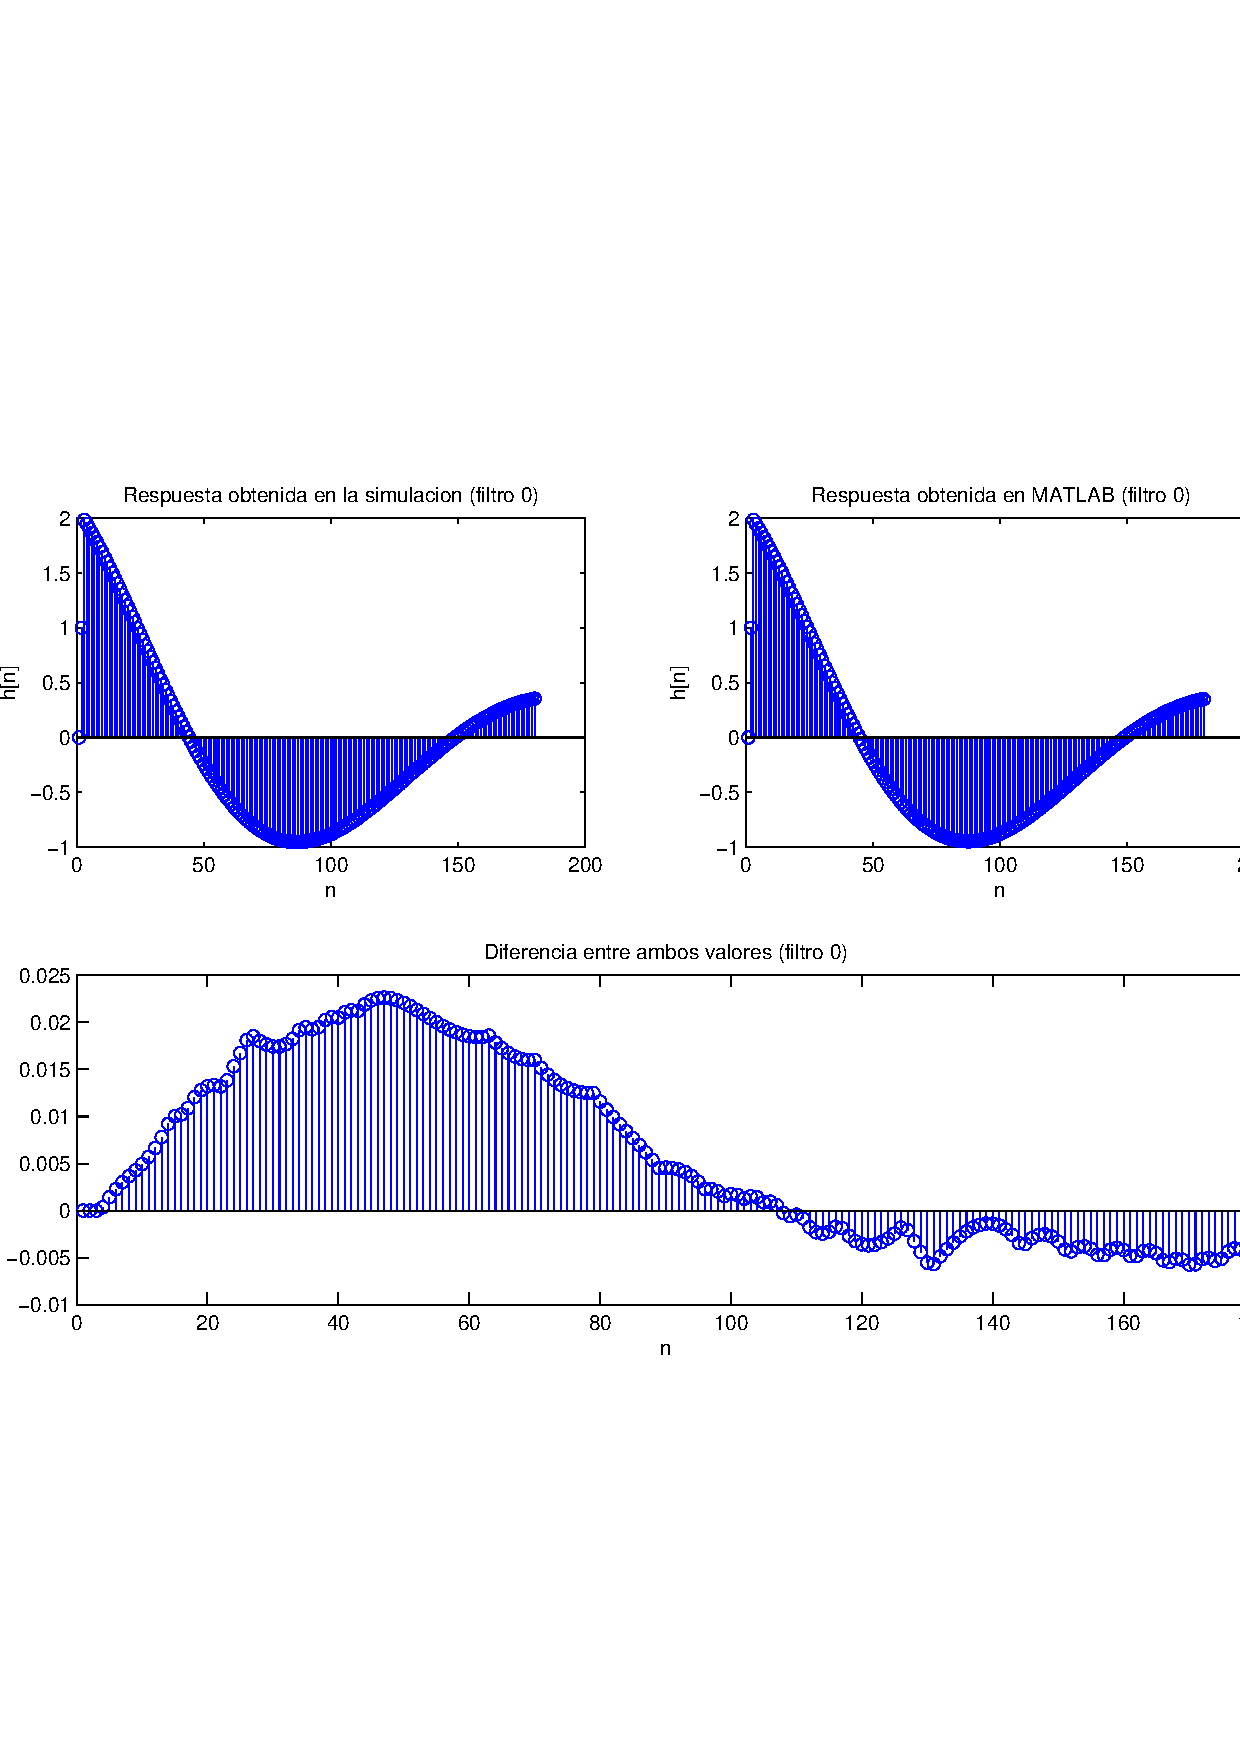
\includegraphics[width=\textwidth]{img/respfiltro0.pdf} 
\caption{Comprobación del filtro 0} \label{fig:filter0}
\end{figure}

\begin{figure}[hbt]
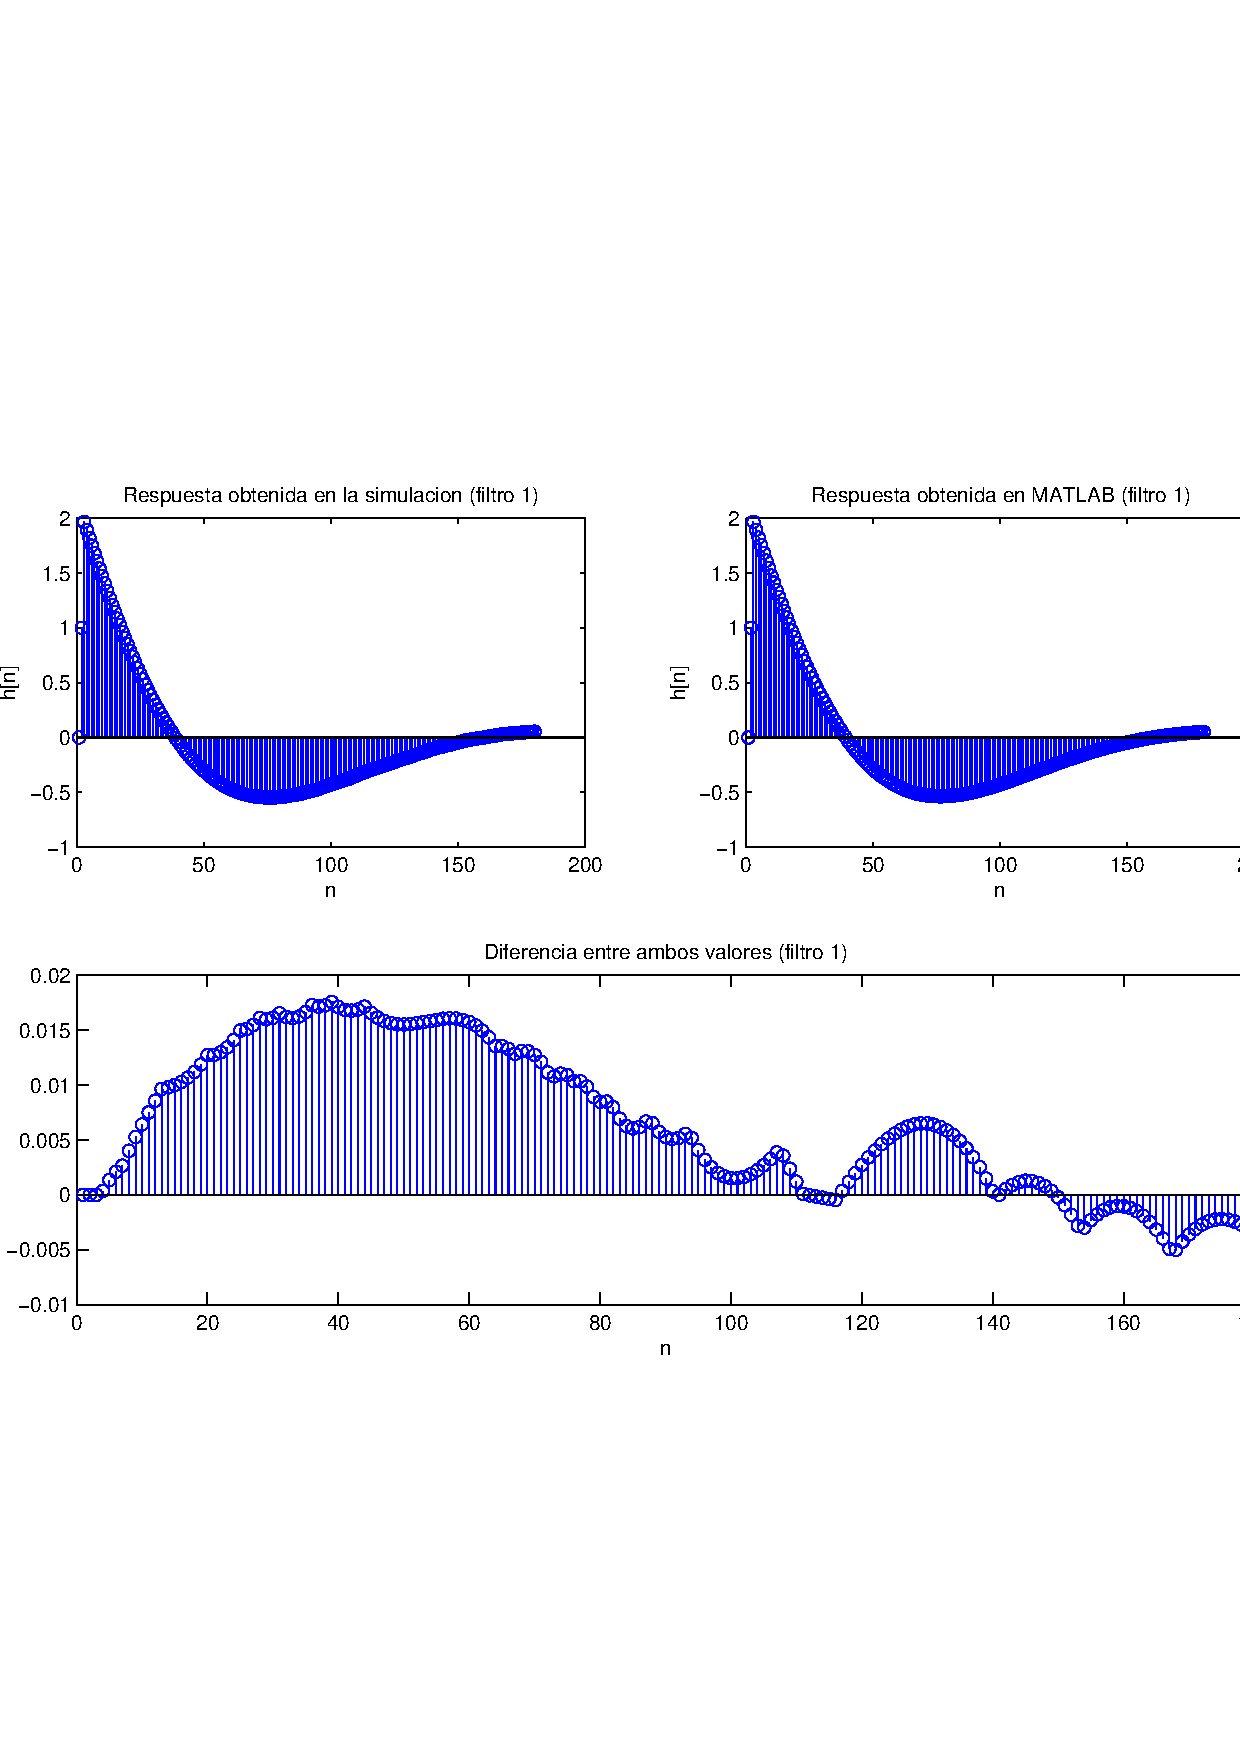
\includegraphics[width=\textwidth]{img/respfiltro1.pdf} 
\caption{Comprobación del filtro 1} \label{fig:filter1}
\end{figure}

\begin{figure}[hbt]
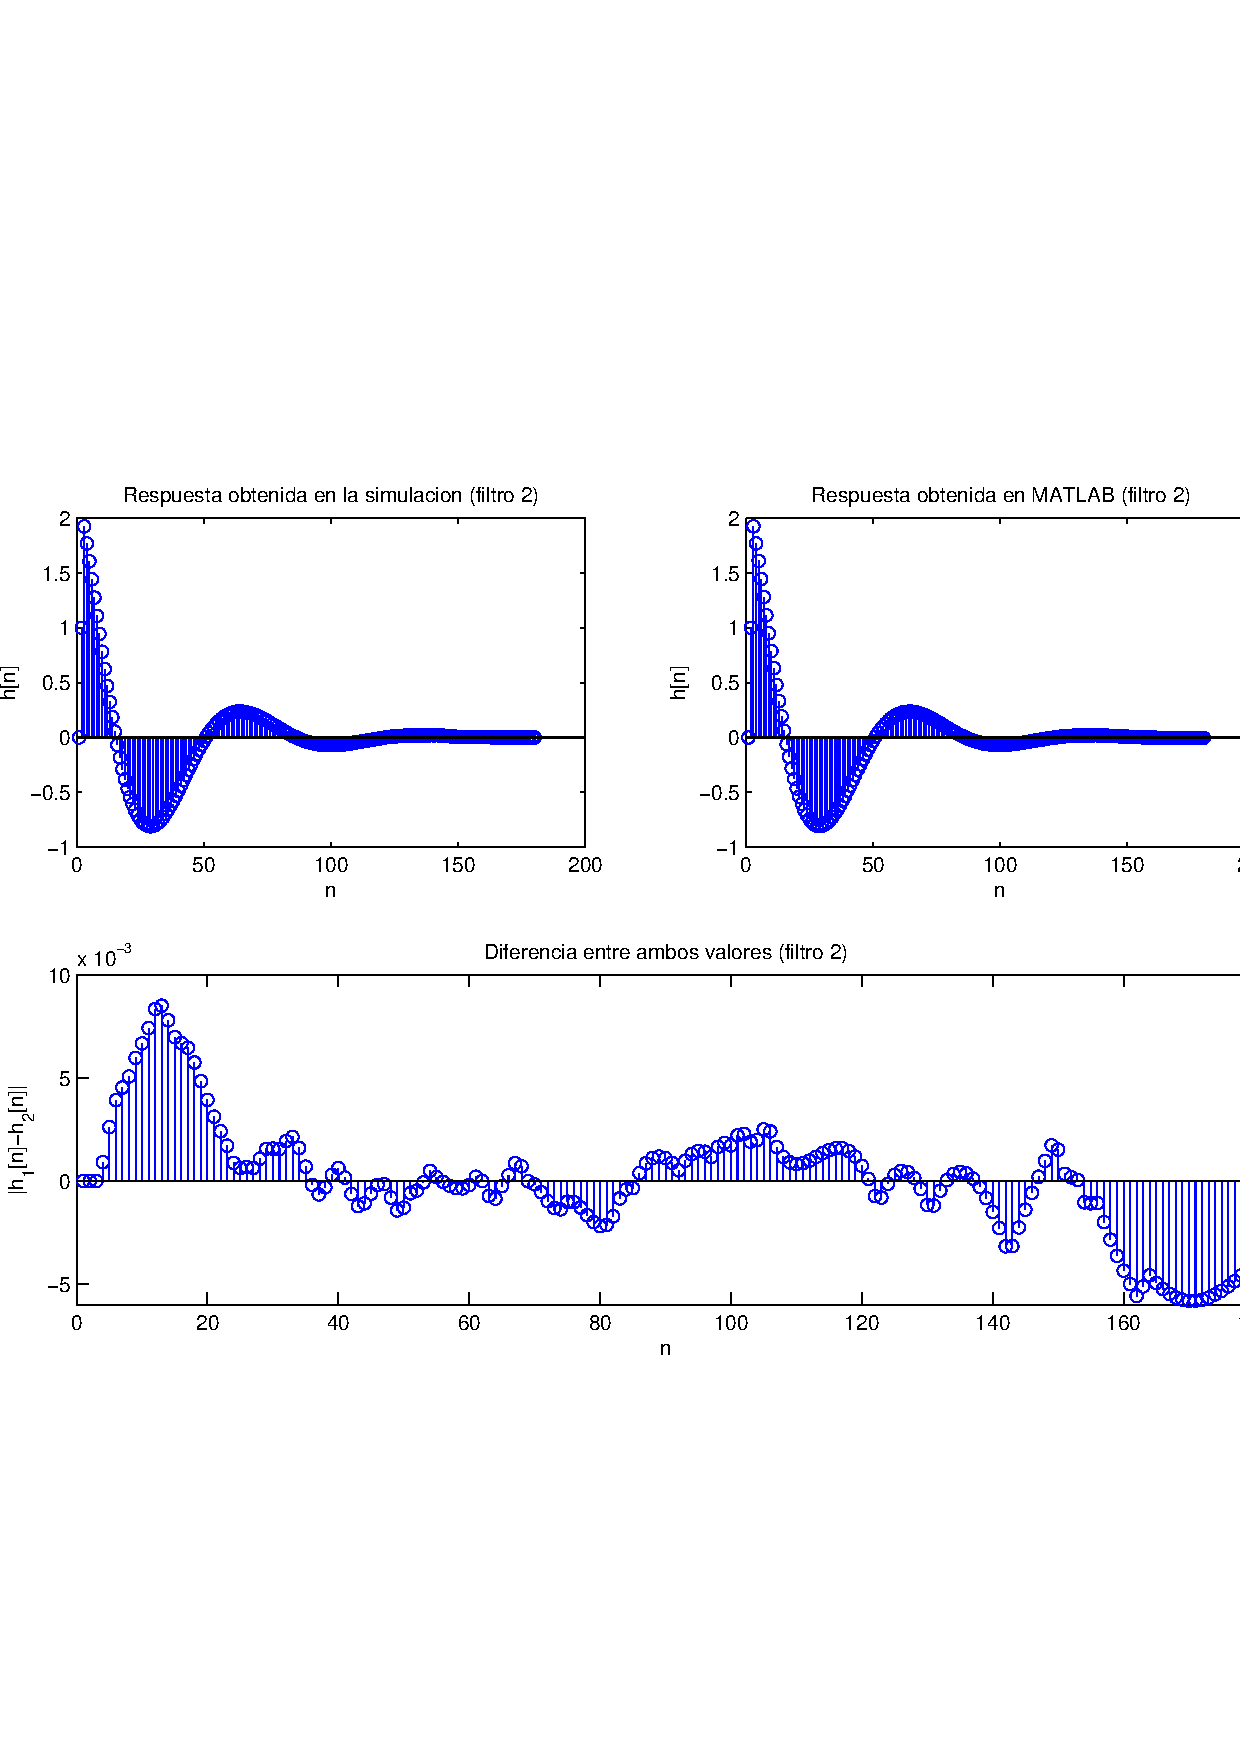
\includegraphics[width=\textwidth]{img/respfiltro2.pdf} 
\caption{Comprobación del filtro 2} \label{fig:filter2}
\end{figure}

\begin{figure}[hbt]
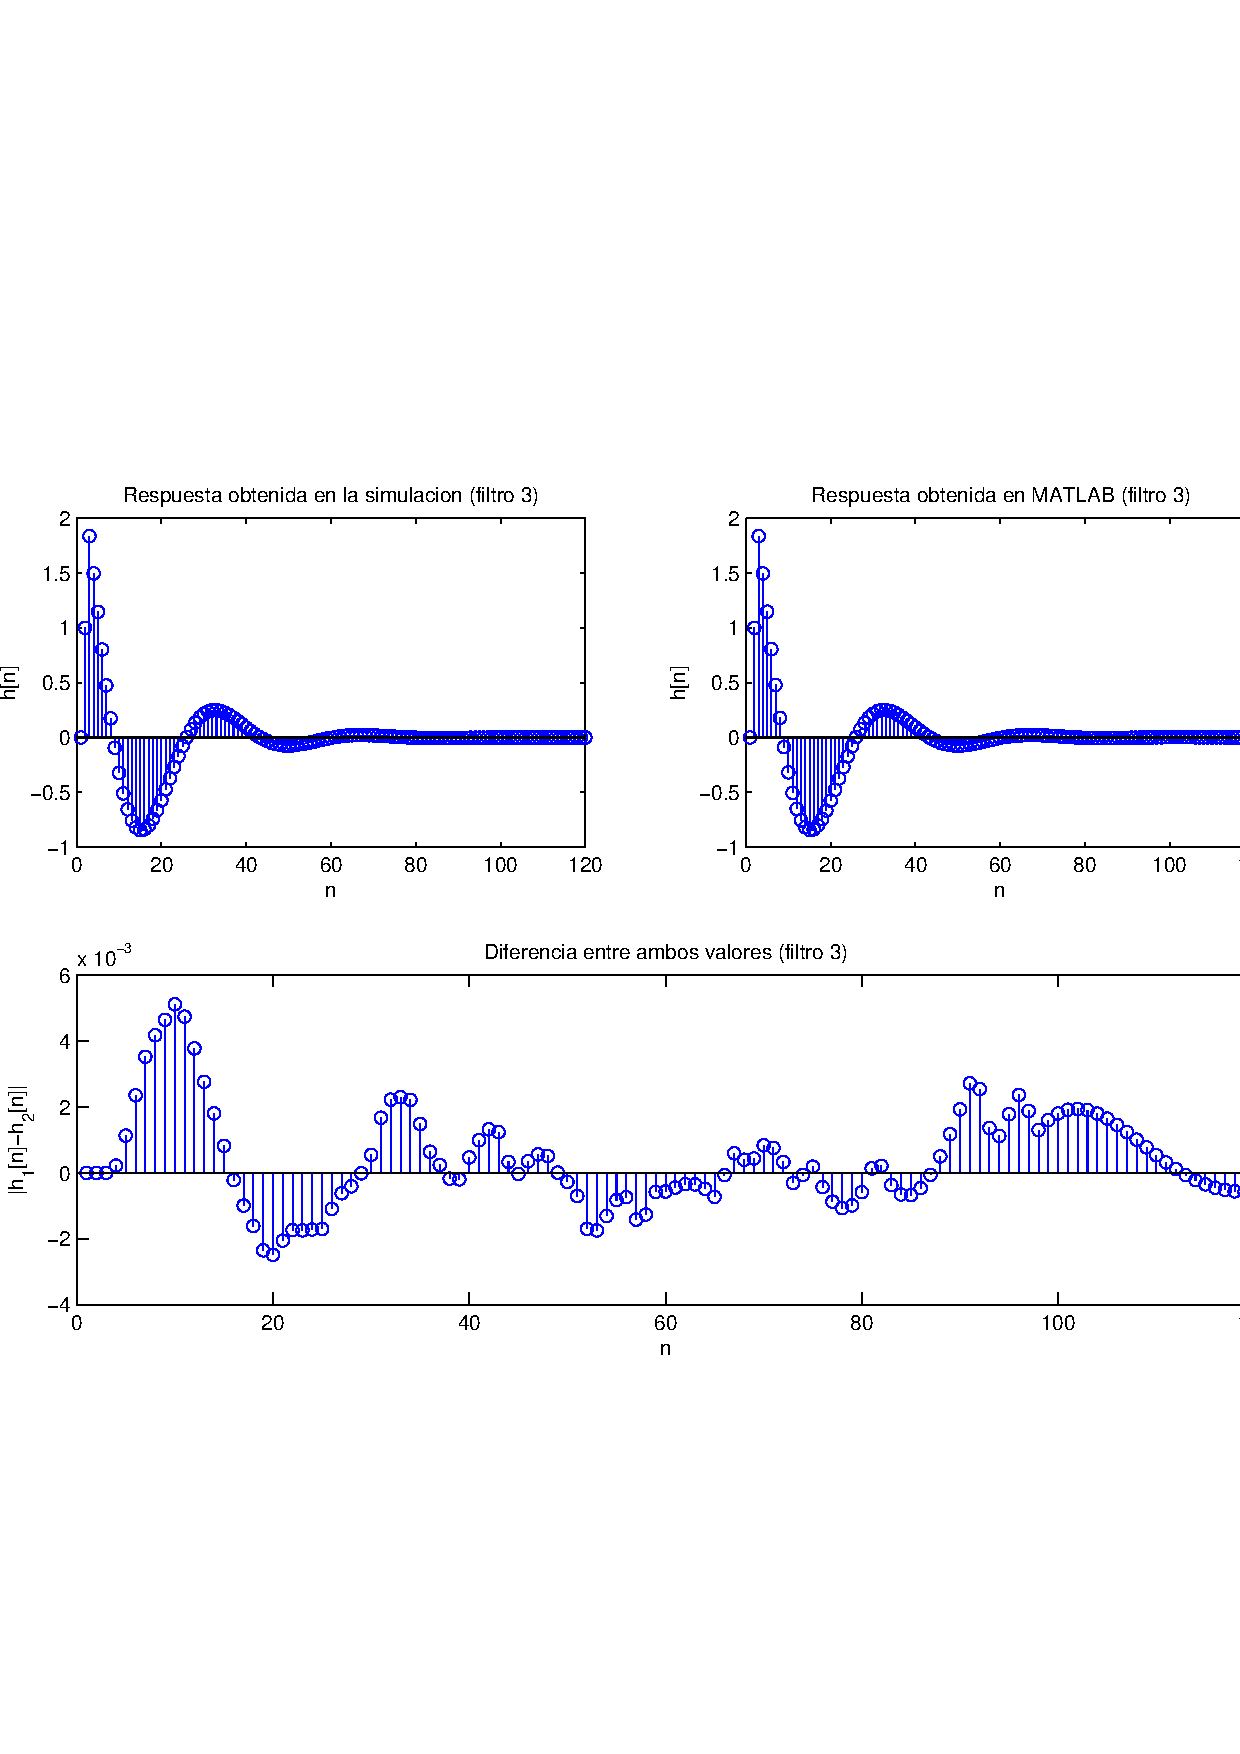
\includegraphics[width=\textwidth]{img/respfiltro3.pdf} 
\caption{Comprobación del filtro 3} \label{fig:filter3}
\end{figure}

\begin{figure}[hbt]
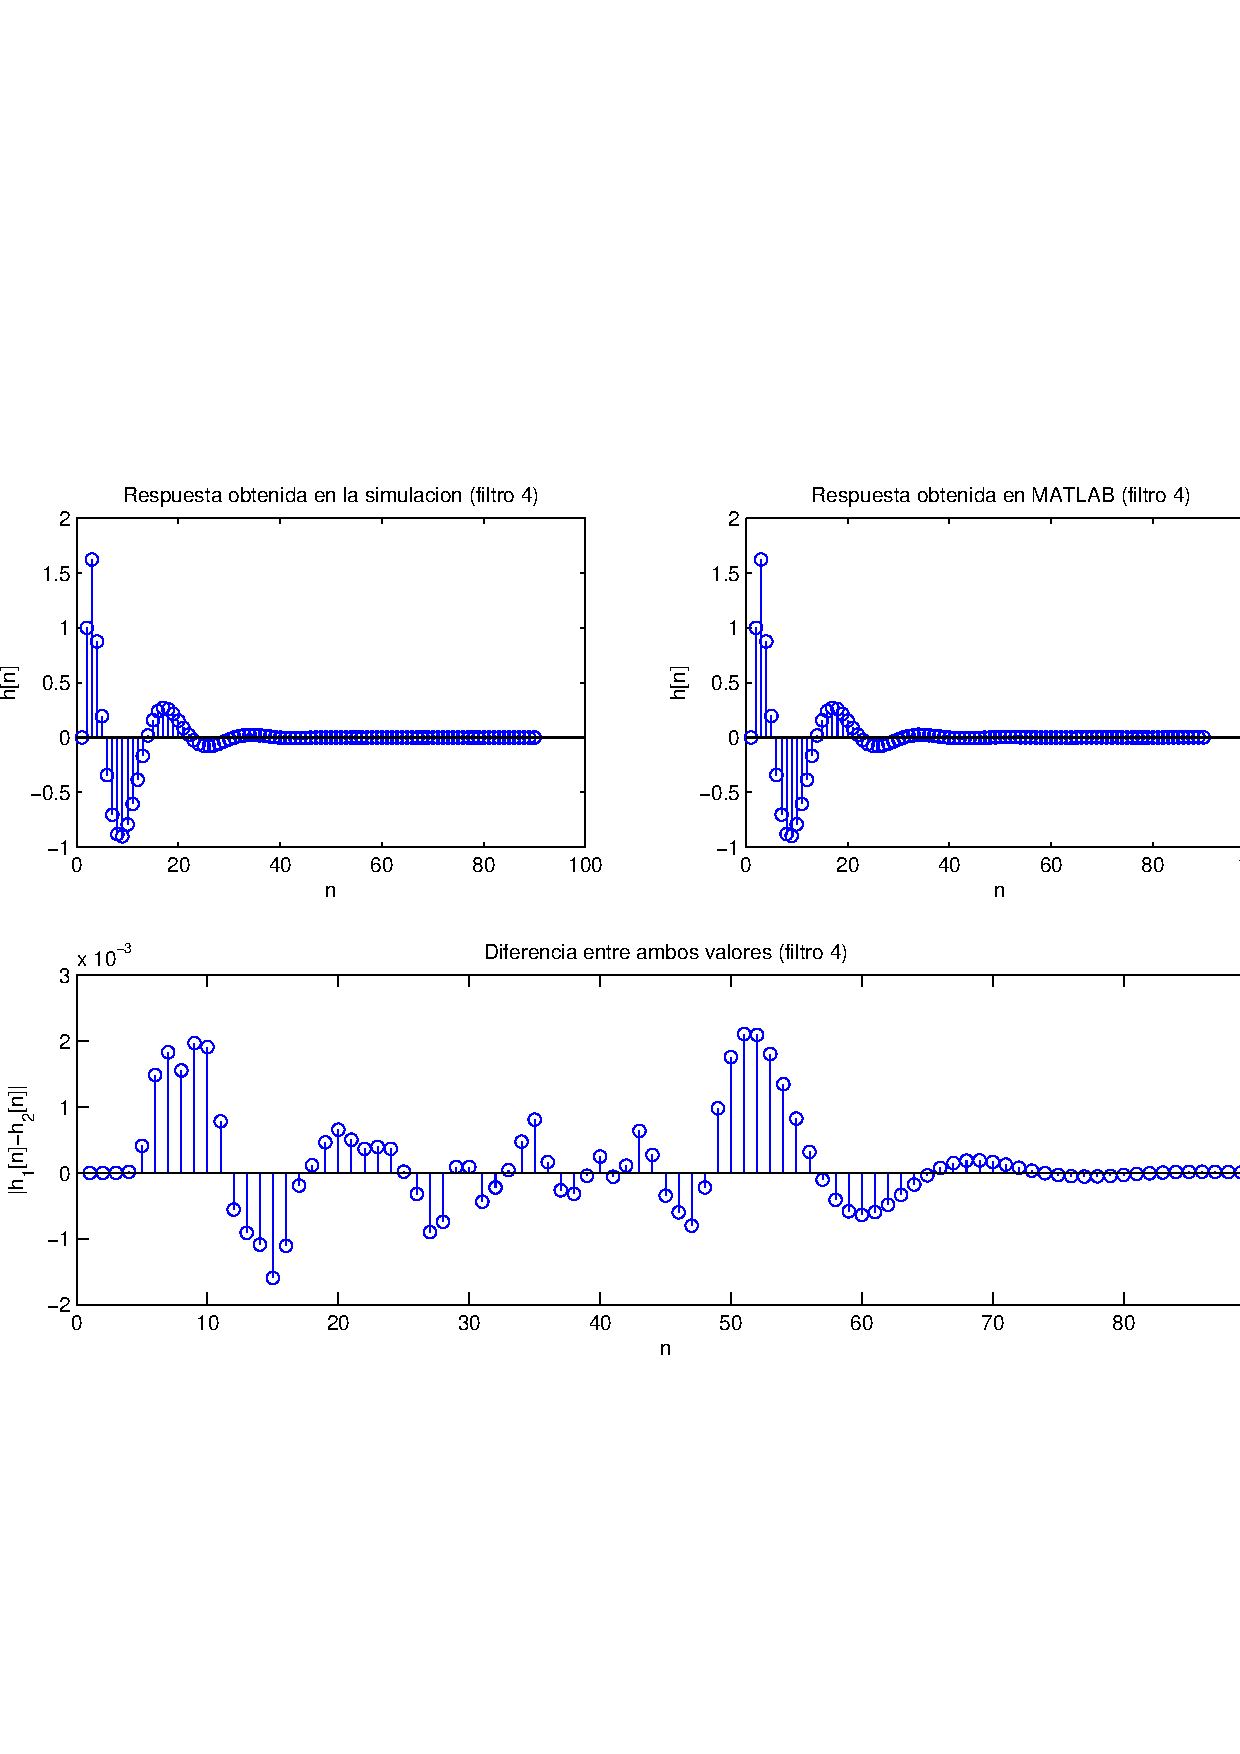
\includegraphics[width=\textwidth]{img/respfiltro4.pdf} 
\caption{Comprobación del filtro 4} \label{fig:filter4}
\end{figure}

\begin{figure}[hbt]
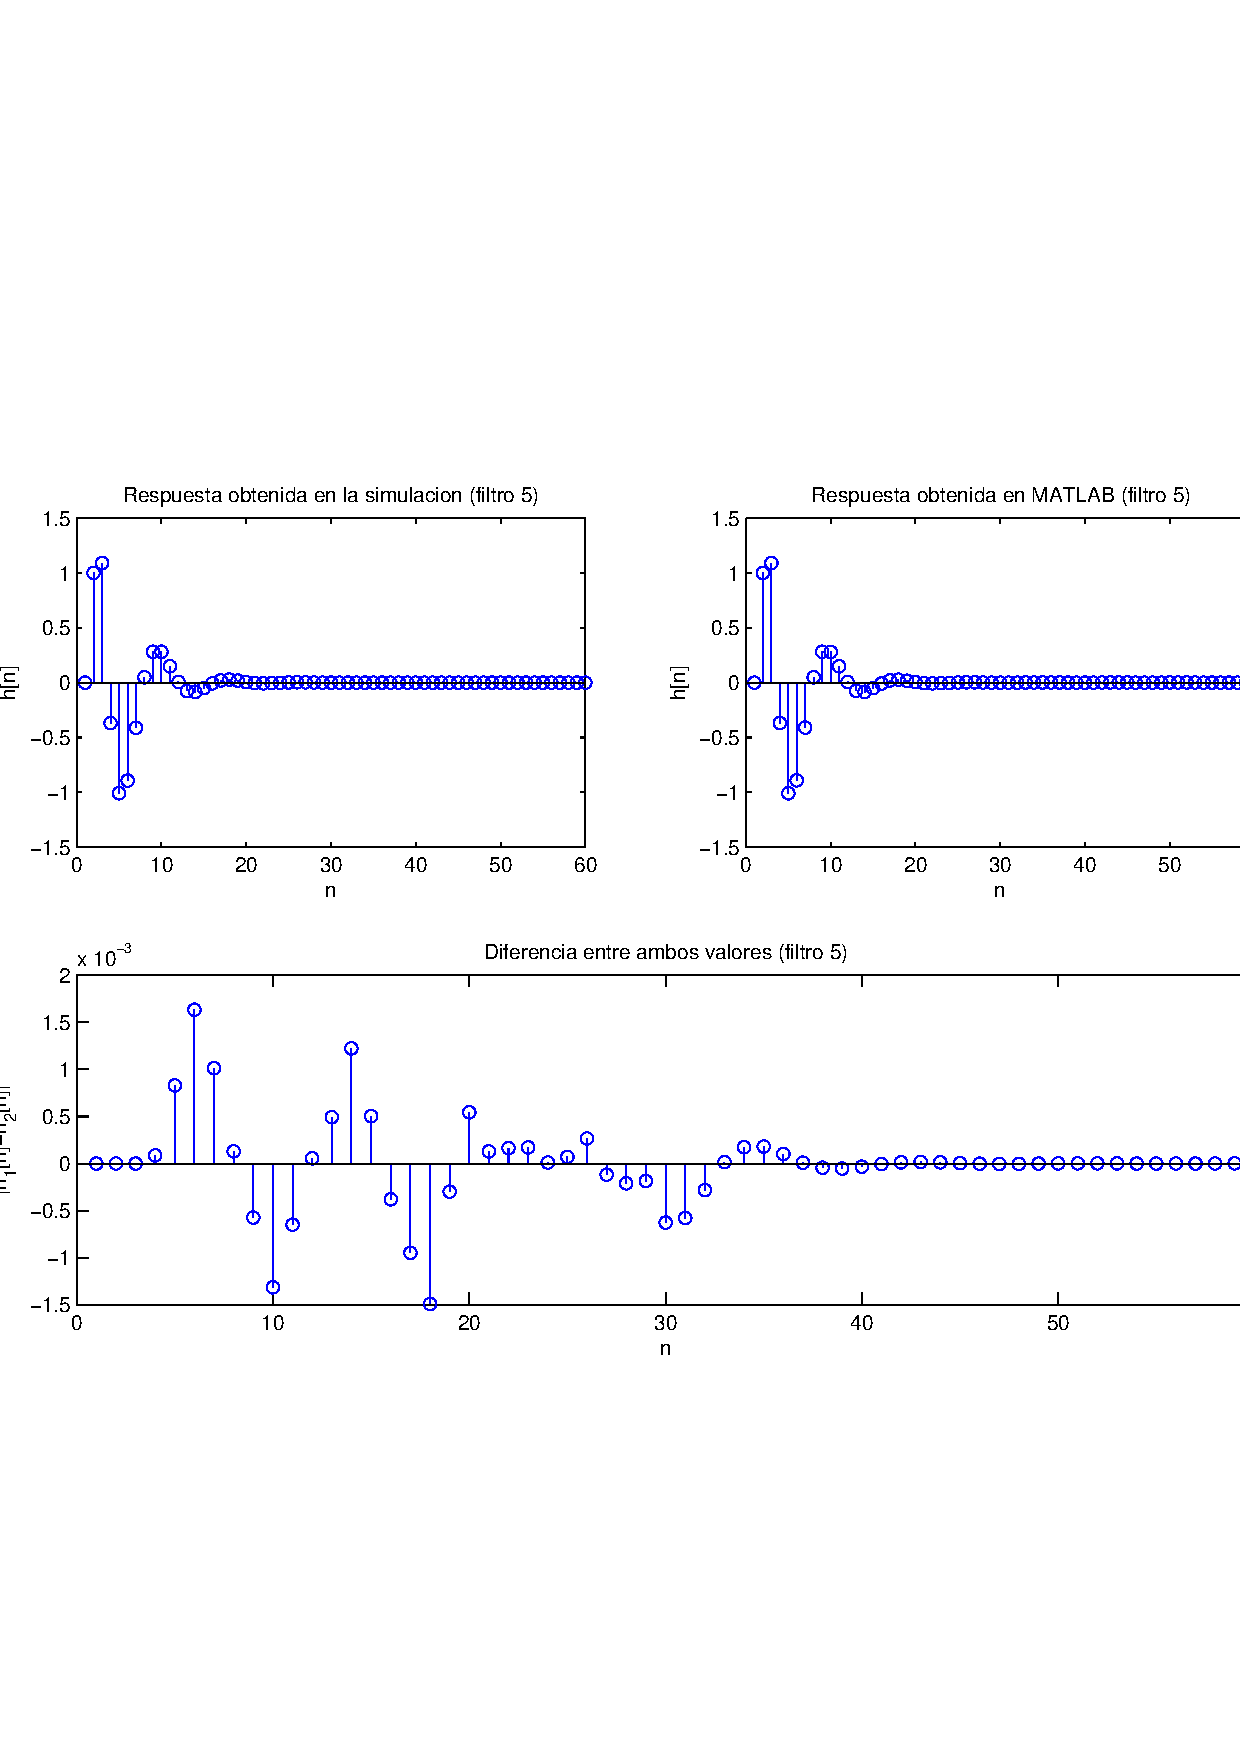
\includegraphics[width=\textwidth]{img/respfiltro5.pdf} 
\caption{Comprobación del filtro 5} \label{fig:filter5}
\end{figure}

\begin{figure}[hbt]
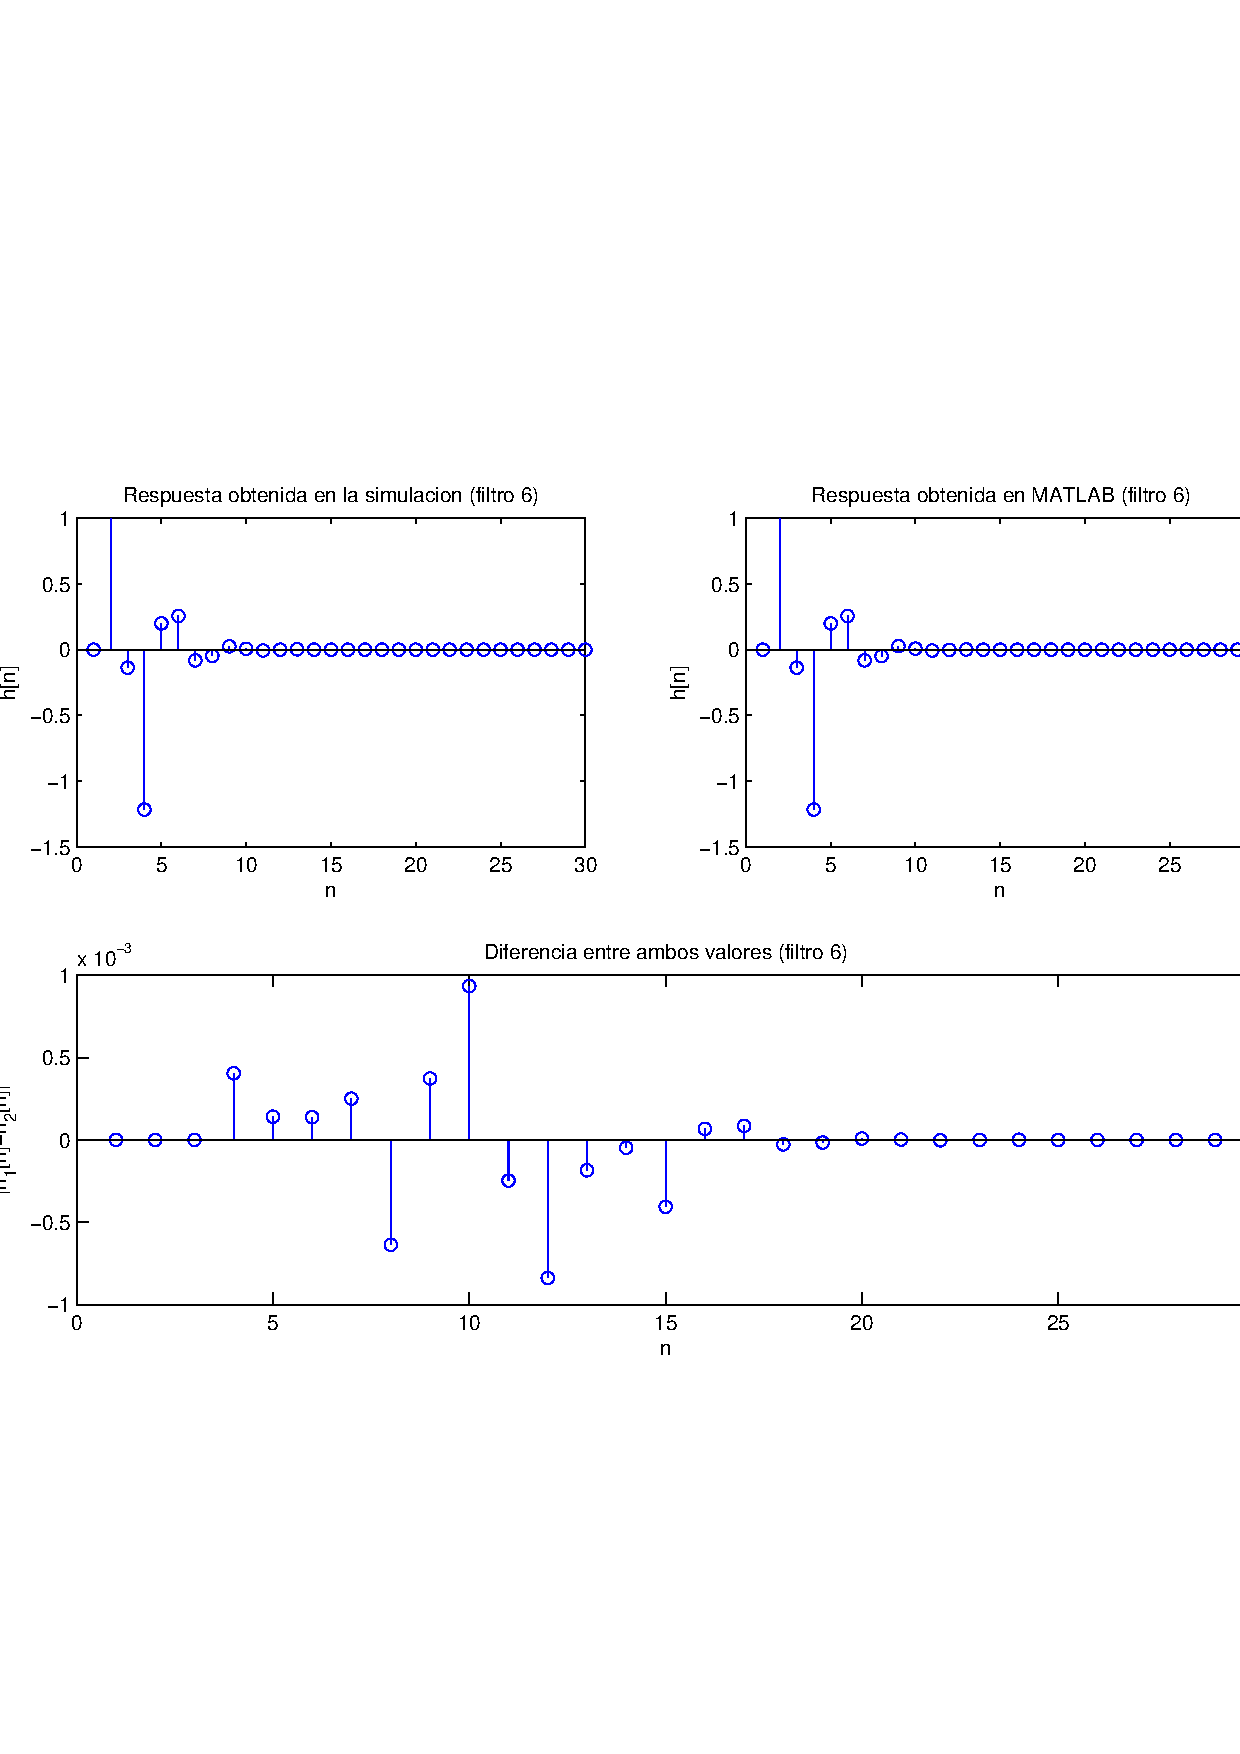
\includegraphics[width=\textwidth]{img/respfiltro6.pdf} 
\caption{Comprobación del filtro 6} \label{fig:filter6}
\end{figure}

\clearpage

\end{document}













